\section{Extended Introduction}
\label{sec:introduction}

\uline{MP splits the model vertically, partitioning the computation and parameters in each layer across multiple devices, requiring significant communication between each layer.} As a result, they work well within a single node where the inter-GPU communication bandwidth is high, but the efficiency degrades quickly beyond a single node \cite{megatronlm}.    

We first analyze the full spectrum of memory consumption of the existing systems on model training and classify it into two parts:  1) For large models, the majority of the memory is occupied by \emph{model states} which include \uline{the optimizer states} (such as momentum and variances in Adam~\cite{DBLP:journals/corr/Adam}), \uline{gradients}, and \uline{parameters}. 
2) The remaining memory is consumed by \uline{activation}, \uline{temporary buffers} and \uline{unusable fragmented memory}, which we refer to collectively as \emph{residual} states.
We develop \name --- Zero Redundancy Optimizer  --- to optimize memory efficiency on both while obtaining high compute and communication efficiency.

{\bf Optimizing Model State Memory:}
DP has good compute/communication efficiency but poor memory efficiency while MP can have poor compute/communication efficiency.
More specifically, \uline{DP replicates the entire model states across all data parallel process resulting in redundant memory consumption};
while \uline{MP partition these states to obtain high memory efficiency, but often result in too fine-grained computation and expensive communication that is less scaling efficient.}
Furthermore, all of these approaches maintain all the model states required over the entire
training process statically, even though not all model states are required all the time during
the training.

\textbf{\name-DP removes the memory state redundancies across data-parallel processes by \emph{partitioning} the model states instead of replicating them, and it retains the compute/communication efficiency by retaining the computational granularity and communication volume of DP using a dynamic communication schedule during training.}

\name-DP has three main optimization stages (as depicted in Figure \ref{fig:memory-consumption}), which correspond to the partitioning of optimizer states, gradients, and parameters. When enabled cumulatively:

\begin{figure}[t!]
 \begin{center}
 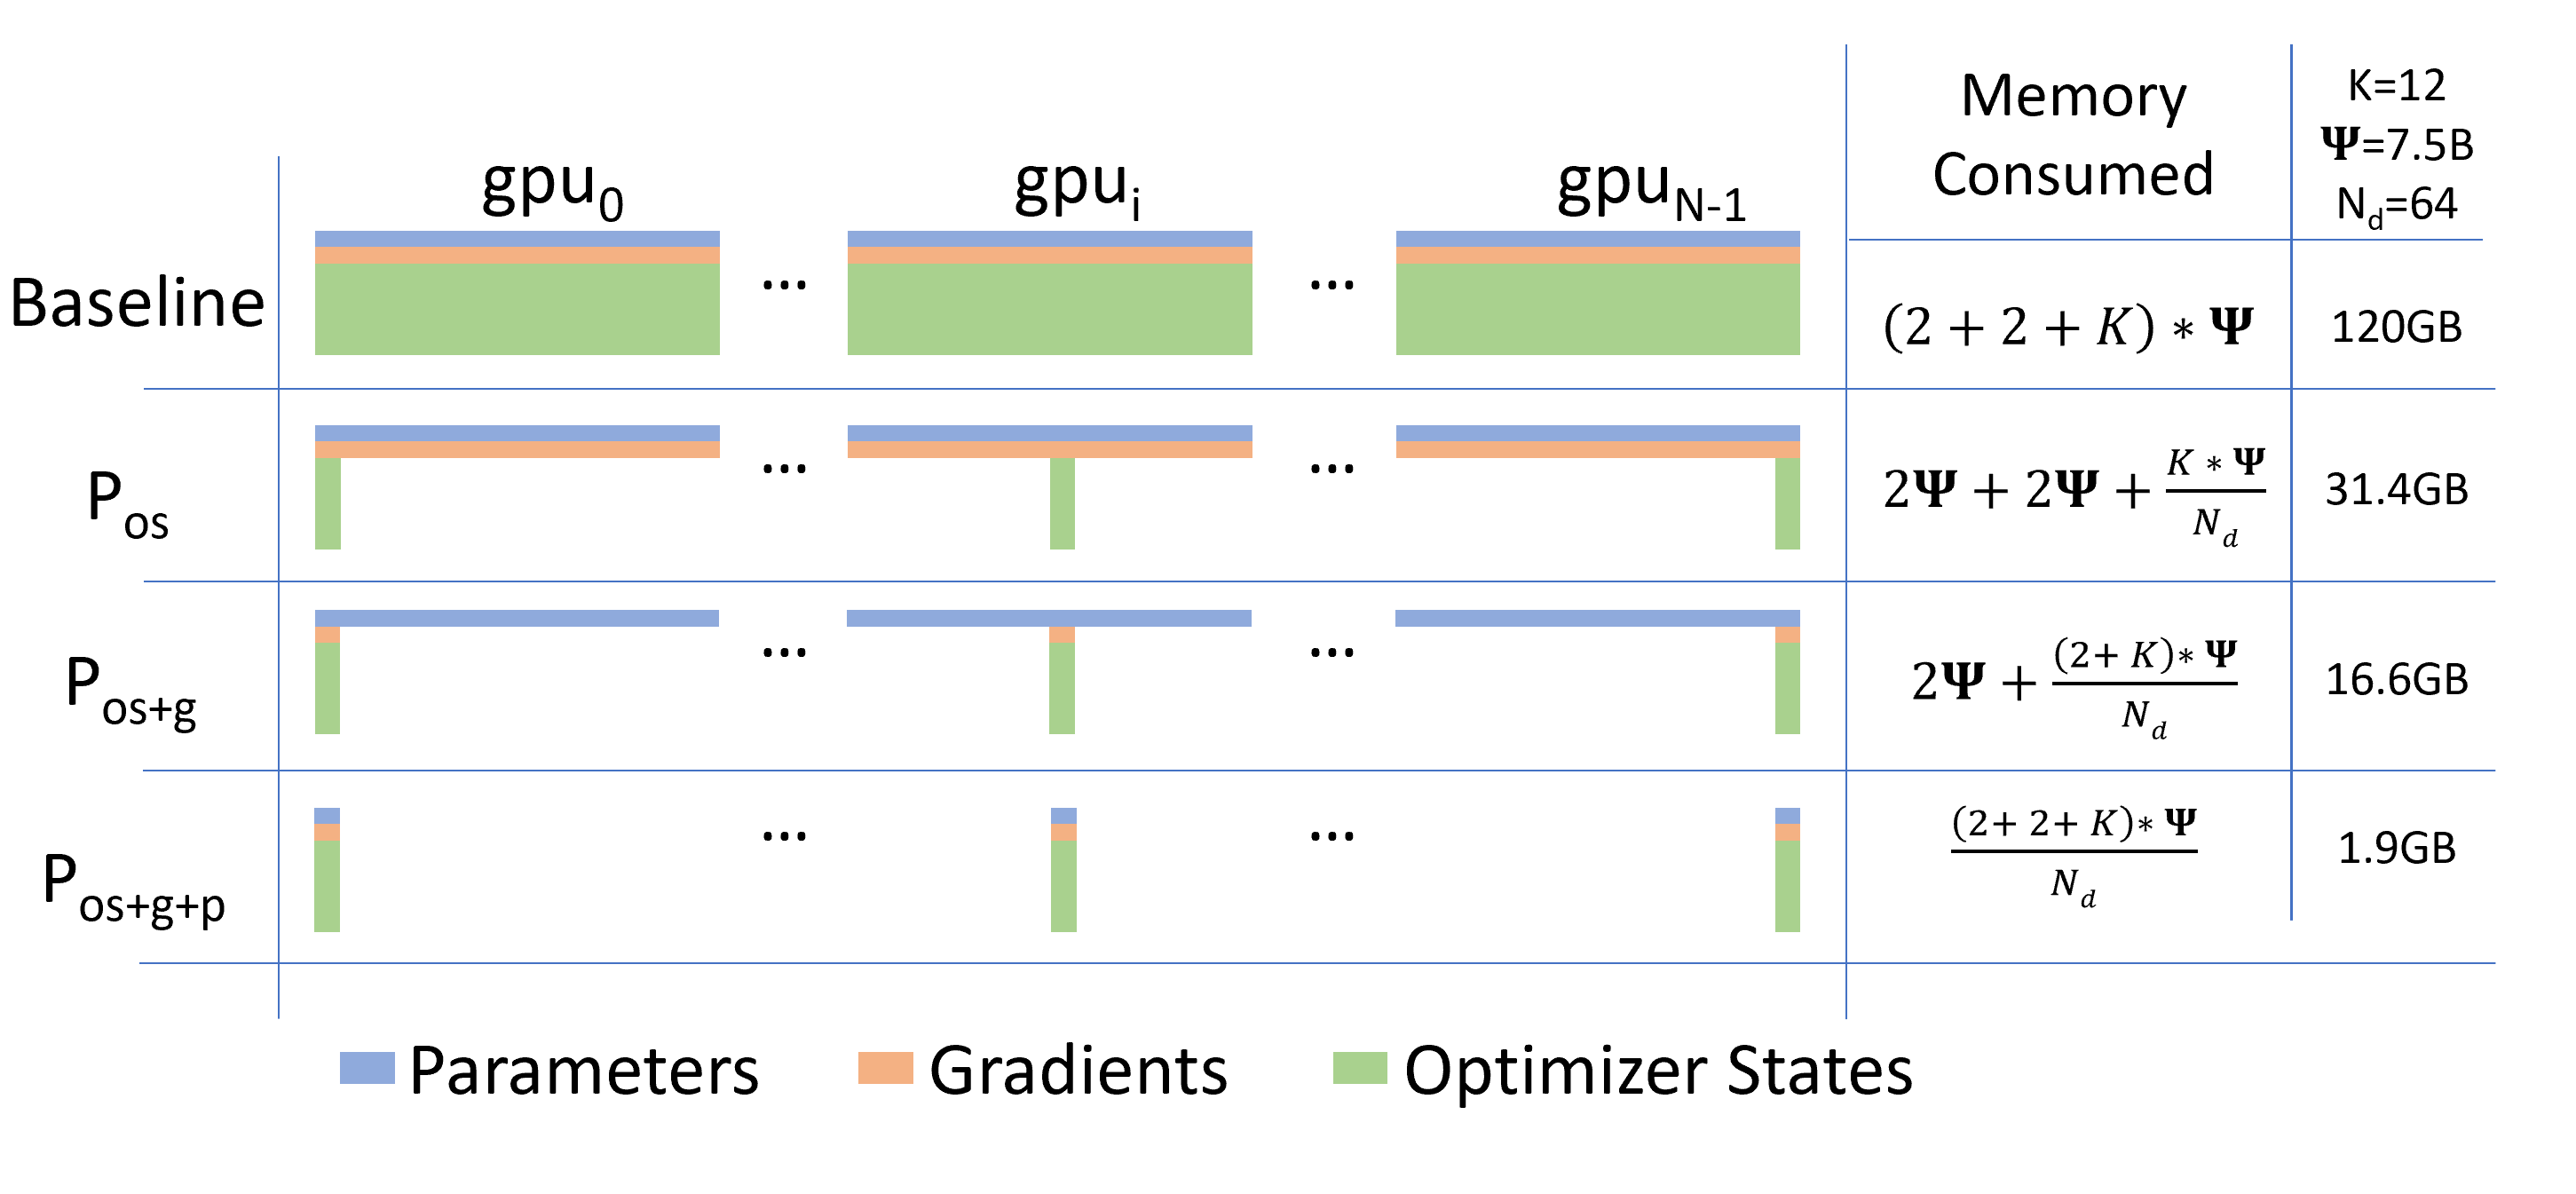
\includegraphics[width=1.0\columnwidth]{memory-consumption-v4.PNG}
 \caption{Comparing the per-device memory consumption of model states, with three stages of \name-DP optimizations. $\Psi$ denotes model size (number of parameters), $K$ denotes the memory multiplier of optimizer states, and $N_d$ denotes DP degree.  In the example, we assume a model size of $\Psi=7.5B$ and DP of $N_d=64$ with $K=12$ based on mixed-precision training with Adam optimizer. } 
 \label{fig:memory-consumption}
 \end{center}
\end{figure}

1) Optimizer State Partitioning ($P_{os}$): \uline{4x memory reduction, same communication volume as DP;}

2) Add Gradient Partitioning ($P_{os+g}$): \uline{8x memory reduction, same communication volume as DP;} 

3) Add Parameter Partitioning ($P_{os+g+p}$): \uline{Memory reduction is linear with DP degree $N_d$.} For example, splitting across 64 GPUs ($N_d$ = 64) will yield a 64x memory reduction. \uline{There is a modest 50\% increase in communication volume.}

{\bf Optimizing Residual State Memory:}
We develop \name-R to optimize the residual memory consumed by these three factors respectively.  

1) For activations (stored from forward pass in order to perform backward pass), we noticed checkpointing \cite{DBLP:journals/corr/ChenXZG16} helps but not sufficient for large models.  
\uline{Thus \name-R optimizes activation memory by identifying and removing activation replication in existing MP approaches through activation partitioning.} \uline{It also offloads activations to CPU when appropriate.}

2) \uline{\name-R defines appropriate size for temporary buffers to strike for a balance of memory and computation efficiency.}

3) We observe fragmented memory during training due to variations in the lifetime of different tensors. Lack of contiguous memory due to fragmentation can cause memory allocation failure, even when enough free memory is available. \uline{\name-R proactively manages memory based on the different lifetime of tensors, preventing memory fragmentation.}

\name-DP and \name-R combined together forms a powerful system of memory optimizations for DL training that we collectively refer to as \name.

There are still cases where we want to leverage MP:

i) \uline{When used with \name-R, MP can reduce activation memory footprint for very large models.}

ii) For smaller models where activation memory is not an issue, MP can also have benefits when aggregated batch size using DP alone is too big to have good convergence.\footnote{Prior work \cite{DBLP:journals/corr/batch-scaling} shows, very large batch size could slow down convergence.  For given model and data, there is a measure of critical-batch size, where increasing batch size further slows down convergence.}  \uline{In those case, one can combine \name with MP to fit the model with an acceptable aggregated batch size.}

We share \name as a part of our open source DL training optimization library called DeepSpeed\footnote{\url{https://github.com/microsoft/deepspeed}}.